\documentclass[11pt]{article}
\usepackage{geometry}                % See geometry.pdf to learn the layout options. There are lots.
\geometry{letterpaper}                   % ... or a4paper or a5paper or ... 
%\geometry{landscape}                % Activate for for rotated page geometry
%\usepackage[parfill]{parskip}    % Activate to begin paragraphs with an empty line rather than an indent
\usepackage{graphicx}
\usepackage{amssymb}
\usepackage{epstopdf}
 \usepackage{cite}
\DeclareGraphicsRule{.tif}{png}{.png}{`convert #1 `dirname #1`/`basename #1 .tif`.png}





\title{Cross-Linguistic Phoneme Embeddings for Computational Historical and Typological Linguistics}
\author{Marlon Betz}
%\date{}                                           % Activate to display a given date or no date

\begin{document}
\maketitle
\newpage
\tableofcontents

\section{Introduction}
Embeddings nowadays build the backbone of every Deep Learning NLP architecture. Due to their capacity to encode a vast amount of latent semantic and syntactic information without the need of previous manual construction, they gave rise to the contemporary Deep Learning boom, i.e. deep neural networks that can capture hidden features in data sets and by that have allowed for huge performance gains in numerous NLP fields. \\While embeddings are currently being used for several linguistic units such as characters\cite{kim2015character,dos2014learning,zhang2015character}, words \cite{mikolov2013efficient,mikolov2013distributed,pennington2014glove} or entire sentences \cite{kiros2015skip}, proper phonemes have been largely been excluded from this trend, although there are some data that would indeed allow for it and research areas where they could be of great use, especially in the fields of Computational Typological and Historical Linguistics, which the current deep learning boom has hardly touched yet. There, even though it is clear that some phonemes share more common features and such form natural classes, they are often treated as pure symbols that share a common distance between each other. Even phoneme representation models that do incorporate phonological features are often hand-crafted \cite{kondrak2000new,rama2016siamese} or include task-specific information that inherently suffer from restricted generalization abilities when used for other tasks \cite{jager2014phylogenetic}. Moreover, those methods usually reduce the number of possible phonemes to a minimum, getting rid of important information such as secondary or co-articulations. \\
In this paper, I will first a discuss a theoretical motivation for using data-driven phoneme embeddings instead of plain symbolic representations or hand-crafted feature encodings. I will then shortly take a look on related research. A big part of this paper will then review several embedding models. I will then discuss intrinsic evaluation methods for the embeddings and use those to compare the performances of the previously described models. This is then followed by a discussion of several use cases that could be interesting for those interested in data-driven approaches to Typological and Historical Linguistics. Finally, I will recapitulate the benefits and drawbacks of phoneme embeddings in a final resume.
\section{Theoretical and Practical Motivation}
\section{Related Research}
Word embeddings have proven to be a reliable tool for several NLP tasks. However, finer grained embedding models that take care of the internal structure of a word have been shown to give similar or even improved performance over traditional word embeddings as they are able to encode morphological \cite{dos2014learning} or semantic \cite{chen2015joint} information even for out-of-vocabulary items \cite{ling2015finding}. This follows the simple idea that since a word can be split up into its respective morphemes that encode morphosyntactic and semantic information, encoding subparts of a word instead of a the whole word should allow for better generalization for unseen words without the need to compute and store vector representations for every word type. 
\section{Embedding Models}
\subsection{Count-based Embedding Models}
\subsubsection{Latent Semantic Analysis}
\subsubsection{GloVe}
\subsubsection{SPPMI}
\subsubsection{SPPMI-SVD}
\subsection{Neural Embedding Models}
\begin{figure}[t]
\centering
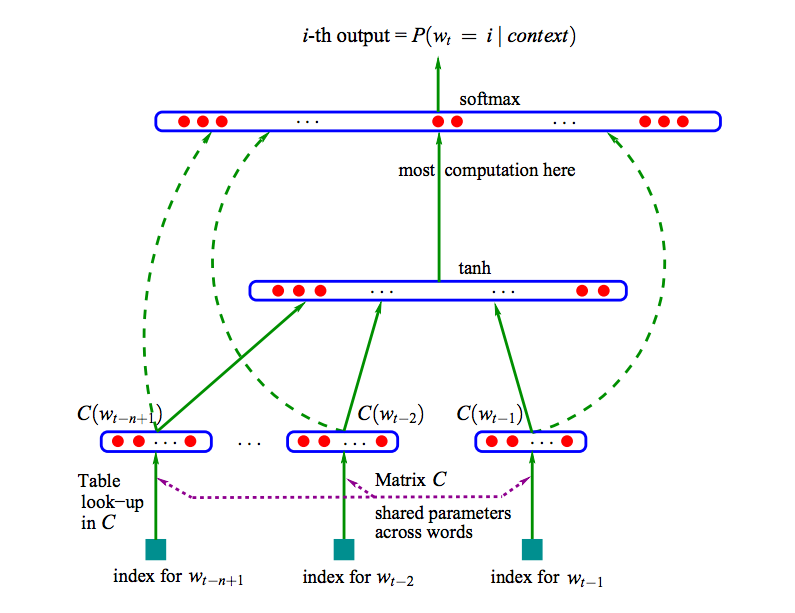
\includegraphics[width=0.75\textwidth]{bengio2006network}
\caption{The neural language model as proposed in \cite{bengio2003neural}.}
\label{fig:bengio2006network}
\end{figure}
Models that make use of  cooccurrence count matrix factorizations usually suffer from the need of storing huge amounts of data into working memory. Neural networks with hidden layers, on the other hand, have been proven to be able to approximate any given hidden function while they still allow for online or mini-batch training. This is a huge improvement over models that only work with whole data batches, as much less working memory has to be used here. \cite{bengio2003neural} pioneered as the first to introduce Neural Language Models in general. Here, a network with two hidden layers is proposed, where a first non-linear hidden layer with locally shared weights gives embeddings of single words in the given context window, while the next layer is a concatenation of the single word embeddings and another non-linear activation function and gives a context embedding. The last layer than is a softmax classifier that predicts the next word (cf. Figure \ref{fig:bengio2006network}). 
It later became clear that this model had two major drawbacks:
\begin{itemize}  
\item The softmax classifier needs to compute the probability of all word types in the vocabulary. This is a major flaw also of following models (see below).
\item The non-linear hidden layer severely worsened the convergence rate of the network.
\end{itemize}
\cite{collobert2008unified} then improved the model tremendously by getting rid of the expensive softmax classifier by introducing a score based loss function: 
\begin{equation}
J_{\theta} = \sum_{x\in X}\sum_{w\in V}\max(0,1-f_{\theta}(x)+f_{\theta}(x^{(w)}))
\label{eq:bengio2006network_loss}
\end{equation}
Here, the the correct windows x containing n words are sampled from the set of all possible windows X in the corpus, while for every window x, a corrupted version $x^{(w)}$ is produced by replacing the center word of $x$ by the another word of the vocabulary $V$. The objective then becomes maximizing the distance between the scores output by the model fore correct and the incorrect window with a margin of 1. The actual model then was still the same as in \cite{bengio2003neural}. This model could already embed semantically similar words close to each other, but still suffered from the non-linear hidden layer, which slowed down learning enormously (\cite{bengio2003neural} report a training time of 7 weeks for a vocabulary of 130000 word types)
\subsubsection{Word2Vec}
\begin{figure}[htbp] %  figure placement: here, top, bottom, or page
   \centering
   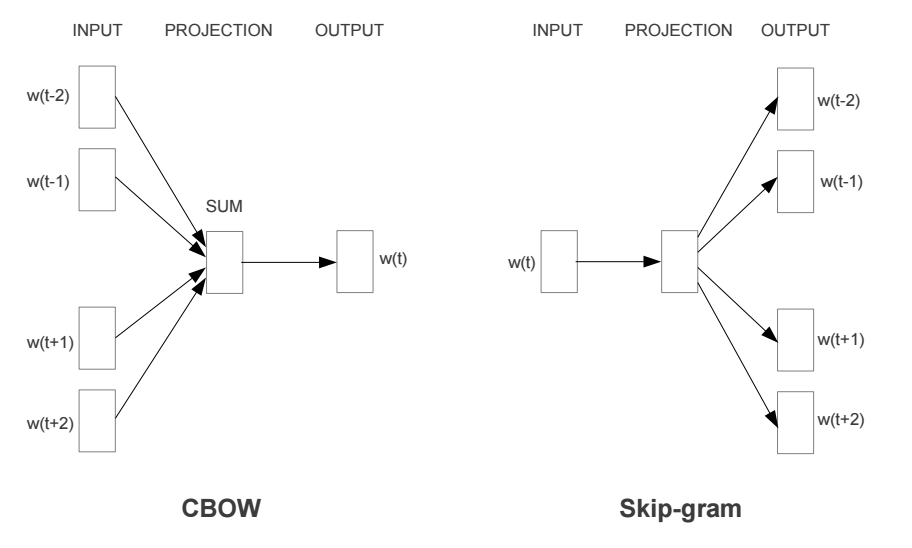
\includegraphics[width=0.75\textwidth]{word2vec} 
   \caption{The two common architectures of word2vec. The Continuous Bag-of-Words (CBOW) model predicts the current word based on the
context, and the Skip-gram predicts surrounding words given the current word. From \cite{mikolov2013efficient}.}
   \label{fig:word2vec}
\end{figure}
Among general-purpose embedding models in general and among neural embedding models in particular, the word2vec algorithm \cite{mikolov2013efficient,mikolov2013distributed} stands out as major breakthrough, as it offers good performance while the parameters to train are less then with the previous models. Different to the previous models in \cite{bengio2003neural,collobert2008unified}, which employ non-linear hidden layers, here the model only consists of a linear encoder layer that computes the actual embeddings. It can be seen as a full departure from traditional embedding models as a subgroup of language models towards a new kind of model family that in the first place tries to encode semantic and morphosyntactic information of a word rather than to predict the next word itself. Instead, the context window usually encompasses all surrounding words of a given target word instead of just the previous words. This makes it rather unhandy for true language modeling, but allows for much better incorporation of latent information. Moreover, the model can be trained in two ways: It either tries to predict the target word given its context (Continuous Bag-of-Words; CBOW) or tries to predict the context of a word given the target word itself (Skip-Gram, cf. Figure \ref{fig:word2vec}). The corresponding loss function for the CBOW model is given as 
\begin{equation}
J_{\theta} = \frac{1}{T} \sum_{t=1}^{T}\log p(w_{t}\mid w_{t-n},\dots,w_{t-1},w_{t+1},\dots,w_{t+n})
\label{eq:CBOW_loss}
\end{equation}

where $p(w_{t}\mid w_{t-1},\dots,w_{t-n+1})$ is given as a softmax

\begin{equation}
p(w_{t}\mid w_{t-1},\dots,w_{t-n+1}) = \frac{\exp(h^\top v'_{w_{t}}))}{\sum_{w_i \in V} \exp(h^\top v'_{w_i})} 
\label{eq:cbow_softmax_prob}
\end{equation}

while the loss for the Skip-Gram model is given as

\begin{equation}
J_{\theta} = \frac{1}{T} \sum_{t=1}^{T}\sum_{-n\leq j\leq n,\neq 0}\log p(w_{t+j}\mid w_{t})
\label{eq:skipgram_loss}
\end{equation}

where $p(w_{t+j}\mid w_{t})$ is again defined as a softmax
\begin{equation}
\log p(w_{t+j}\mid w_{t}) = \frac{\exp(v_{w_{t}}^\top v'_{w_{t+j}}))}{\sum_{w_i \in V} \exp(h^\top v'_{w_i})}
\label{eq:skipgram_softmax_prob}
\end{equation}
where $v_w_i$ is an input vector and $v'_w_i$ an output vector representation of a word $w_i$ and $h^\top$ the transpose of the sum of the output vectors of the words in the context. Again, the calculation of the softmax here includes summing over all contexts in the corpus, which computationally is expensive. Further research largely concentrated on finding a way to define $p$ as a memory- and time-friendly approximation of the true softmax probability. A first solution was given by using a hierarchical softmax classifier \cite{morin2005hierarchical} nstead. Here, the classifier layer is a binary tree with the actual words as leaves. At every node, the network learns to either follow the left or the right branch with a certain probability as in Eq. \ref{eq:skipgram_softmax_prob} that is equal to the sum of the child elements of the respective  branch, but is actually computed as the product of $h^\top$ and the output vector of the word at node $n$ pulled through a logistic sigmoid:

\begin{equation}
p(right|n,c) = \sigma(h^\top v'_n) 
\label{eq:hierarchicalsoftmax_nodeprob}
\end{equation}

This means  in order to calculate the softmax probability of word, we only have to follow the path down to the word leaf instead of summing over all vocabulary entries. For binary trees, this means we only have to pass at most $\log_2(\mid V\mid)$ nodes to calculate the probability of a word, which is a huge performance boost over the traditional softmax classifier.





\section{Evaluation}
\subsection{Data}
\subsection{Evaluation Methods}
\subsection{Results}
\section{Use Cases}
\subsection{Phonemic String Comparison}
\subsection{Modeling Sound Change}
\subsection{Phoneme Inventory Clustering}
\section{Resume}


\bibliographystyle{apa}
\bibliography{references} 


\end{document}  